\section{ผลลัพธ์ประสิทธิภาพการทำงานระหว่าง HAPS และ Terrestrial Networks}

\subsection{วิเคราะห์การนำวิธี ICM เข้าไปใช้ในเทคโนโลยี HAPS}

\begin{multicols}{2}
สาเหตุของสัญญาณรบกวนนั้น เกิดจากข้อจำกัดปริมาณการส่งข้อมูลใน 1 ชุดคำสั่ง (Protocol)
HAPS กระจายสัญญาณครอบคลุมในพื้นที่วงกว้าง จึงทำให้ไม่สามารถแยกแยะความถี่ในแต่ละคลื่นสัญญาณได้
การสื่อสารระหว่างสัญญาณจาก HAPS ไปยังสถานีภาคพื้นดินหลัก (Base Station - BS)
และอุปกรณ์รับสัญญาณของผู้ใช้งานทั่วไป เช่น Smartphone (User Equipment - UE) \ref{fig:04-haps-with-tn}

\begin{itemize}
    \item Type 1 - เกิดสัญญาณรบกวนเป็นหลักที่ฝั่ง UE
    \item Type 2 - เกิดสัญญาณรบกวนเล็กน้อยที่ฝั่ง H-UE
    \item Type 3 - สัญญาณ Uplink เกิดสัญญาณรบกวนเล็กน้อยที่ฝั่ง H-UE แสดงให้เห็นว่าการปรับทิศทางส่งสัญญาณส่งผล
    ต่อการลดสัญญาณรบกวน
    \item Type 4 - การส่งสัญญาณจากสถานีหลัก(Base Station - BS) ไป HAPS Uplink
\end{itemize}

ผลการทดลองทั้ง 4 Type สรุปได้ว่าสัญญาณที่ส่งจากสถานีหลักไปยัง HAPS ด้วยการปรับมุมและทิศทางสามารถช่วยลดโอกาสที่จะเกิดสัญญาณรบกวนและลดปริมาณทรัพยากรที่ใช้ และประเมินผลออกมาเป็นกราฟดังนี้
\ref{fig:04-haps-compare-downlink}

กราฟแสดงถึงผลที่เกิดจากสัญญาณรบกวนจาก HAPS ไปยังสถานีภาคพื้นดิน (TN) และอุปกรณ์ของผู้ใช้ (UE)
ในความถี่และรัศมีครอบคลุมที่แตกต่างกัน (2 GHz, 39 GHz, 0 km., 100 km.) โดยมีตัวชี้วัดคือประสิทธิภาพของสเปกตรัม(Spectral Efficiency - SE)
วัดปริมาณข้อมูลที่ส่งผ่านแบนด์วิธ (bandwidth) ภายในระบบ

\columnbreak


\begin{figure}[H]
\centering
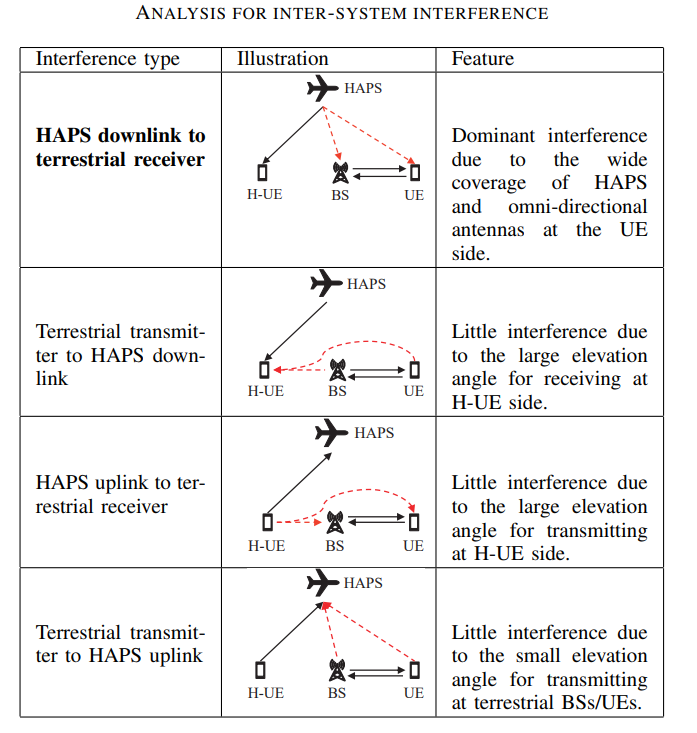
\includegraphics[width=0.3\textwidth]{04_haps-with-tn.png}
\caption[Interference Type]{Analysis for Inter-System Interference} \label{fig:04-haps-with-tn} 
\end{figure}

\begin{figure}[H]
\centering
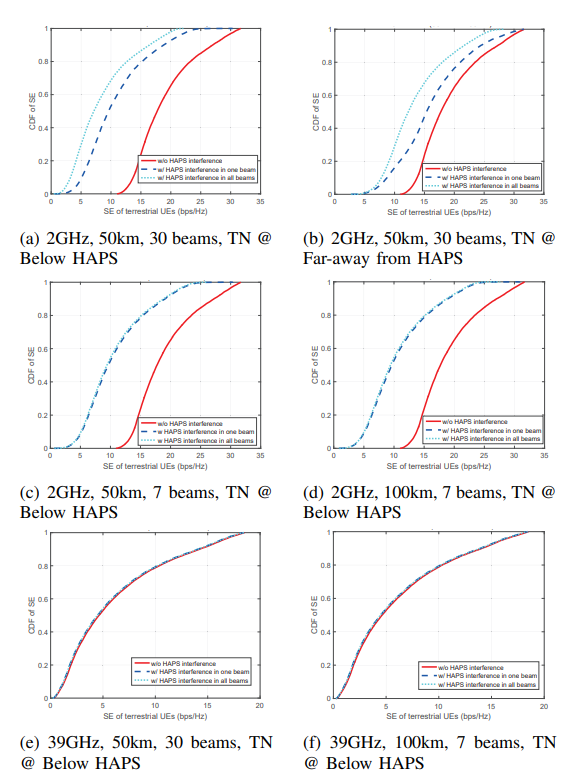
\includegraphics[width=0.3\textwidth]{04_haps-compare-downlink.png}
\caption[HAPS compare with downlink]{Downlink SE performance in terrestrial network (TN) with or without
the interference from HAPS downlink.} \label{fig:04-haps-compare-downlink}
\end{figure}
\end{multicols}

\pagebreak

\subsection{การปรับใช้}

แบ่งออกเป็น 2 กรณีคือ กรณี Baseline 1 โดย HAPS และเครือข่ายภาคพื้นดิน (TN) ใช้ทรัพยากรเดียวกันโดยไม่คำนึงถึงปริมาณการรับส่งข้อมูล 
หมายความว่าทรัพยากรนั้นไม่ได้มีการจัดสรรแบบไดนามิกตามปริมาณการรับส่งข้อมูล ส่วนในกรณี Baseline 2 HAPS และเครือข่ายภาคพื้นดินสัญญาณได้มีการจัดสรรทรัพยากรที่ความถี่ที่ 5 และ 15 MHz 
แสดงให้เห็นว่าทั้งสองระบบมีการจัดสรรทรัพยากรคงที่แต่คนละวิธี ทำให้การนำวิธีแทรกคลื่นสัญญาณ (ICM) มาปรับใช้ช่วยแก้ปัญหาในเรื่องทรัพยากร
และเพิ่มประสิทธิภาพการทำงานในทั้งสองเครือข่าย จากรูป \ref{fig:05-avg-thruput-full-freq} HAPS ในกรณี Baseline 2 ให้ผลลัพธ์ที่สูงกว่า Baseline 1 
สำหรับผู้ใช้ที่อยู่ในขอบเขตของ HAPS ในขณะที่ Baseline 1 ให้ผลลัพธ์ได้ดีกว่าสำหรับผู้ใช้ที่อยู่นอกขอบเขตของHAPS โดยการทำงานมีประสิทธิภาพสูงสุดใน layer 2
และ layer 3 จากรูป \ref{fig:05-avg-thruput-5-cl-freq} การส่งข้อมูลด้วยความถี่ 5-color ใน HAPS มีประสิทธิภาพในการทำงานคล้ายกับความถี่แบบสูงสุด

โดยรวมแล้วเราสรุปผลในทาง techical terms ออกมาได้ดังตารางต่อไปนี้ \ref{table:04-haps-evaluation}

\begin{table}[h]
\centering
% 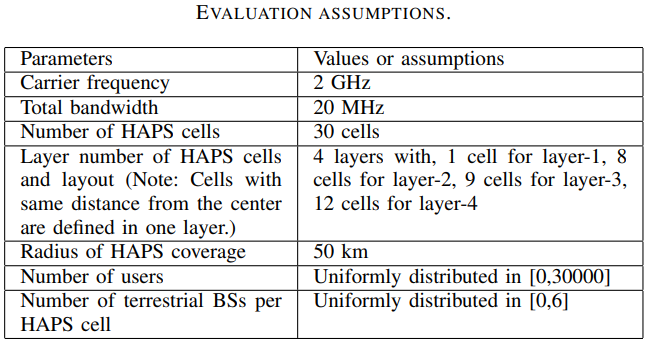
\includegraphics[width=0.5\textwidth]{04_haps_evaluation.png}
\begin{tabular}[h]{| l | l |}
\hline
Parameters                      & Values or assumptions \\
\hline
Carrier frequency               & 2 GHz \\
\hline
Total bandwidth                 & 20 MHz \\
\hline
Number of HAPS cells            & 30 cells \\
\hline
\parbox[t]{12em}{Layer number of HAPS cells and layout (Note: Cells with same distance from the center are defined in one layer.)}        & \parbox[t]{12em}{4 layers with, 1 cell for layer-1, 8 cells for layer-2, 9 cells for layer-3, 12 cells for layer-4} \\
\hline
Radius of HAPS coverage         & 50 km \\
\hline
Number of users                 & Uniformly distributed in [0,30000] \\
\hline
Number of terrestrial BSs per HAPS cell & Uniformly distributed in [0,6]\\
\hline
\end{tabular}
\caption{Evaluation Assumptions} \label{table:04-haps-evaluation}
\end{table}

\subsection{การประยุกต์ใช้ ICM}

จากงานวิจัยของ \cite[Interference Coordination Method for Integrated HAPS-Terrestrial Networks]{liu2021interference}
นำเสนอถึงวิธีการแทรกคลื่นสัญญาณ (Interference Coordination Method - ICM) เข้าไประหว่างคลื่นสัญญาณของ HAPS กับ สถานีเครือข่ายภาคพื้นดิน โดยมีเงื่อนไขต่อไปนี้
\begin{itemize}
    \item คำนึงถึงการกระจายปริมาณรับส่งข้อมูลเป็นหลัก 
    \item ประสิทธิภาพที่ได้โดยเทียบจากปริมาณพลังงาน,ทรัพยากรที่เสียไปและปริมาณข้อมูลที่เคลื่อนที่ผ่านเครือข่าย ณ เวลาที่กำหนด (Traffic Load)
\end{itemize}
